% ============================================================
% BAB IV — HASIL DAN PEMBAHASAN
% ITERA Smart Sentinel: Sistem Deteksi & Analitik Pelanggaran Helm Real-time
% ============================================================

\chapter{HASIL DAN PEMBAHASAN}
\label{chap:hasil}

Bab ini menyajikan hasil penelitian beserta pembahasannya dalam dua bagian terpisah agar pembaca dapat membedakan paparan data lapangan dari penafsiran maknanya. Sub-bab~\ref{sec:hasil} memuat data mentah yang sudah diolah dalam bentuk tabel, gambar, dan deskripsi numerik tanpa diberi opini. Sub-bab~\ref{sec:pembahasan} membahas makna data tersebut, membandingkannya dengan teori dan penelitian terdahulu yang dirujuk pada Bab Tinjauan Pustaka, serta menonjolkan kebaruan yang dihasilkan penelitian ini. Susunan tiga aspek penelitian, yaitu pengembangan model deteksi YOLOv8, \textit{pipeline streaming} deteksi waktu nyata, serta \textit{data mart} dan visualisasi analitik, dijaga paralel di kedua sub-bab supaya alur penalaran mudah diikuti.

% ============================================================
\section{Hasil}
\label{sec:hasil}
% ============================================================

Sub-bab ini melaporkan tiga kelompok temuan secara berurutan, sejalan dengan tahapan metodologi pada Bab~\ref{chap:metodologi}. Kelompok pertama menyajikan karakteristik dataset, parameter pelatihan, dan metrik kinerja model YOLOv8. Kelompok kedua melaporkan keluaran tiap tahap \textit{pipeline} \textit{streaming} ketika diuji pada potongan 3.001 \textit{frame} video gerbang utama Itera. Kelompok ketiga melaporkan volume \textit{data mart}, waktu eksekusi kueri, dan tampilan \textit{dashboard} hasil rekaman operasional 10 jam.

% ------------------------------------------------------------
\subsection{Hasil Pengembangan Model Deteksi YOLOv8}
\label{subsec:hasil-model}
% ------------------------------------------------------------

\subsubsection{Karakteristik Dataset dan Sebaran Spasial Anotasi}
\label{subsubsec:hasil-eda}

Dataset mentah hasil tangkapan CCTV memuat 390 citra unik berukuran median $1280 \times 720$ piksel dengan total 2.369 anotasi objek atau rata-rata 6,1 anotasi per citra. Tabel~\ref{tab:distribusi-objek} merinci distribusi anotasi pada setiap kelas.

\begin{table}[htbp]
  \centering
  \caption{Jumlah anotasi tiap kelas pada dataset awal.}
  \label{tab:distribusi-objek}
  \begin{tabular}{clc}
    \hline
    \textbf{No.} & \textbf{Kategori Objek} & \textbf{Jumlah Anotasi} \\
    \hline
    0 & \texttt{DRIVER\_HELMET}     & 730 \\
    1 & \texttt{DRIVER\_NO\_HELMET} & 718 \\
    2 & \texttt{MOTORCYCLE}         & 921 \\
    \hline
    \textbf{Total} & & \textbf{2.369} \\
    \hline
  \end{tabular}
\end{table}

Tabel~\ref{tab:distribusi-objek} memuat tiga kelas dengan jumlah anotasi yang relatif berdekatan. Kelas \texttt{DRIVER\_HELMET} dan \texttt{DRIVER\_NO\_HELMET} hanya berselisih 12 anotasi atau rasio 1{,}02$:$1, sedangkan \texttt{MOTORCYCLE} sebagai kelas konteks memuat 921 anotasi. Rasio kelas mayoritas terhadap kelas minoritas adalah 921$:$718 atau 1{,}28$:$1.

Selain dari sisi jumlah, posisi kemunculan objek pada bidang pandang kamera diperiksa melalui peta panas (\textit{annotation heatmap}). Gambar~\ref{fig:heatmap-per-class} menampilkan kepadatan \textit{bounding box} pada setiap \textit{grid} citra dengan gradasi biru muda hingga merah pekat. Nilai minimum, kuartil pertama, dan median pada legenda sama-sama 0 anotasi, kuartil ketiga 11 anotasi, sedangkan \textit{grid} terpadat memuat 172 anotasi.

\begin{figure}[htbp]
  \centering
  \includegraphics[width=0.95\textwidth]{gambar/heatmap_anotation_class.png}
  \caption{Peta panas (\textit{annotation heatmap}) sebaran anotasi tiap kelas: a) \texttt{DRIVER\_HELMET}, b) \texttt{DRIVER\_NO\_HELMET}, dan c) \texttt{MOTORCYCLE}.}
  \label{fig:heatmap-per-class}
\end{figure}

Pada Gambar~\ref{fig:heatmap-per-class}(a), anotasi kelas \texttt{DRIVER\_HELMET} mengumpul di bagian tengah hingga kanan atas citra dengan titik paling padat di lajur masuk utama. Pola sebaran kelas \texttt{DRIVER\_NO\_HELMET} pada Gambar~\ref{fig:heatmap-per-class}(b) hampir sama, hanya saja zona terpadatnya sedikit bergeser ke kiri tengah. Gambar~\ref{fig:heatmap-per-class}(c) untuk kelas \texttt{MOTORCYCLE} memperlihatkan zona kepadatan yang nyaris sama dengan kelas \texttt{DRIVER\_HELMET}. Di luar zona-zona padat, warna peta panas didominasi biru muda hingga abu-abu yang menandakan \textit{grid} kosong, mencakup langit, trotoar, dan jalur berlawanan di tepi citra.

\subsubsection{Hasil Pra-pemrosesan dan Augmentasi Data}
\label{subsubsec:hasil-preprocessing}

Pra-pemrosesan dan augmentasi mengubah 390 citra mentah menjadi 856 sampel pelatihan terstandarisasi. Setiap citra dikalibrasi dengan \textit{auto-orient}, lalu diubah ukurannya ke resolusi seragam $640 \times 640$ piksel. Tahap augmentasi menghasilkan tiga variasi sintetis untuk setiap citra asli melalui enam teknik: rotasi $\pm 8^\circ$, \textit{shear} $\pm 0{,}2$ pada sumbu X dan Y, \textit{exposure} $\pm 10\%$, \textit{Gaussian blur} \textit{kernel} 1 piksel, \textit{additive noise} 1\%, dan \textit{motion blur} 10 piksel. Citra sebelum dan sesudah augmentasi ditampilkan pada Gambar~\ref{fig:aug-rotasi}--\ref{fig:aug-noise}.

\begin{figure}[H]
  \centering
  \includegraphics[width=0.85\textwidth]{gambar/aug_rotasi.png}
  \caption{Augmentasi rotasi pada rentang $-8^\circ$ sampai $+8^\circ$.}
  \label{fig:aug-rotasi}
\end{figure}

\begin{figure}[H]
  \centering
  \includegraphics[width=0.95\textwidth]{gambar/aug_shear.png}
  \caption{Augmentasi \textit{shear} pada sumbu X dan Y dengan nilai $\pm 0{,}2$.}
  \label{fig:aug-shear}
\end{figure}

\begin{figure}[H]
  \centering
  \includegraphics[width=0.95\textwidth]{gambar/aug_exposure.png}
  \caption{Augmentasi \textit{exposure} pada rentang $-10\%$ sampai $+10\%$.}
  \label{fig:aug-exposure}
\end{figure}

\begin{figure}[H]
  \centering
  \includegraphics[width=0.95\textwidth]{gambar/aug_blur.png}
  \caption{Augmentasi \textit{Gaussian blur} dengan \textit{kernel} 1 piksel.}
  \label{fig:aug-blur}
\end{figure}

\begin{figure}[H]
  \centering
  \includegraphics[width=0.8\textwidth]{gambar/aug_noise.png}
  \caption{Augmentasi \textit{additive noise} sebesar 1\% dari total piksel.}
  \label{fig:aug-noise}
\end{figure}

Citra hasil rotasi pada Gambar~\ref{fig:aug-rotasi} memperlihatkan horizon citra ikut berubah mengikuti sudut $-8^\circ$ sampai $+8^\circ$. Empat varian \textit{shear} pada Gambar~\ref{fig:aug-shear} memiringkan citra pada sumbu X dan Y. Pada Gambar~\ref{fig:aug-exposure}, citra dengan eksposur $-10\%$ tampak lebih gelap dengan bayangan dominan, sedangkan eksposur $+10\%$ membuat citra lebih cerah dengan kontras yang menurun. Gambar~\ref{fig:aug-blur} memperlihatkan tepi objek yang sedikit kabur namun bentuk objek tetap dapat dibedakan, sementara Gambar~\ref{fig:aug-noise} menampilkan bintik halus yang mengaburkan detail tepi tanpa mengubah bentuk keseluruhan.

\subsubsection{Konfigurasi Pelatihan dan Dinamika Kurva Galat}
\label{subsubsec:hasil-training}

Dataset yang sudah diperluas dibagi dengan rasio 82\% pelatihan (699 citra), 9\% validasi (79 citra), dan 9\% pengujian (78 citra). Pelatihan berjalan selama 300 \textit{epoch} pada layanan terkelola Roboflow Train 3.0 varian \textit{Roboflow 3.0 Object Detection (Fast)} yang berbasis arsitektur YOLOv8n (lihat Sub-bab~\ref{subsec:pelatihan-yolov8n}). Pelatihan memantau tiga komponen galat: \textit{box loss} (kesalahan posisi dan ukuran \textit{bounding box}), \textit{class loss} (kesalahan klasifikasi kelas), dan \textit{distribution focal loss} atau DFL (kesalahan distribusi posisi tepi \textit{bounding box}). Gambar~\ref{fig:train-loss} memuat kurva pada data pelatihan, dan Gambar~\ref{fig:val-loss} memuat kurva pada data validasi.

\begin{figure}[H]
\centering
\includegraphics[width=\textwidth]{gambar/train_loss.jpg}
\caption{Dinamika \textit{train loss} model YOLOv8 selama 300 \textit{epoch}: (A) \texttt{train/box\_loss}, (B) \texttt{train/cls\_loss}, dan (C) \texttt{train/dfl\_loss}.}
\label{fig:train-loss}
\end{figure}

Gambar~\ref{fig:train-loss} panel (A) memperlihatkan \texttt{train/box\_loss} turun dari sekitar 2,0 di \textit{epoch} awal hingga sekitar 0,5 menjelang \textit{epoch} 300, dengan penurunan paling tajam dalam 30 \textit{epoch} pertama. Panel (B) memperlihatkan \texttt{train/cls\_loss} jatuh tajam dari 4,0 ke sekitar 1,0 dalam 10 \textit{epoch} pertama, lalu melandai sampai sekitar 0,4 di akhir pelatihan. Panel (C) memperlihatkan \texttt{train/dfl\_loss} bergerak dari 1,55 menuju 0,83 dengan penurunan lebih landai dibanding dua kurva sebelumnya.

\begin{figure}[H]
\centering
\includegraphics[width=\textwidth]{gambar/val_loss.jpg}
\caption{Dinamika \textit{validation loss} model YOLOv8 selama 300 \textit{epoch}: (A) \texttt{val/box\_loss}, (B) \texttt{val/cls\_loss}, dan (C) \texttt{val/dfl\_loss}.}
\label{fig:val-loss}
\end{figure}

Gambar~\ref{fig:val-loss} panel (A) memperlihatkan \texttt{val/box\_loss} dimulai pada kisaran 1,4--1,5 dan masih bergejolak pada 30--90 \textit{epoch} pertama dengan beberapa lonjakan ke atas 1,5. Mulai \textit{epoch} 150, kurva mendatar di sekitar 0,99 dan bertahan sampai \textit{epoch} 300. Panel (B) menunjukkan \texttt{val/cls\_loss} turun tajam dari 3,5 ke 1,0 sebelum \textit{epoch} 30 lalu melandai sampai sekitar 0,6 di akhir pelatihan. Panel (C) menampilkan \texttt{val/dfl\_loss} sempat turun dari 1,15 ke kisaran 1,05--1,10 dalam 60 \textit{epoch} pertama, lalu merangkak naik ke kisaran 1,15--1,16 hingga \textit{epoch} 300.

\subsubsection{Hasil Evaluasi Kinerja Model}
\label{subsubsec:hasil-evaluasi}

Kinerja model dinilai pada himpunan validasi (\textit{validation set}) memakai tiga metrik utama: \textit{Mean Average Precision} pada ambang IoU 50\% (mAP@50), \textit{precision}, dan \textit{recall}. Ringkasannya disajikan di Tabel~\ref{tab:metrik-validasi}.

\begin{table}[htbp]
\centering
\caption{Ringkasan metrik model YOLOv8 pada data validasi.}
\label{tab:metrik-validasi}
\begin{tabular}{lc}
\toprule
\textbf{Metrik} & \textbf{Nilai} \\
\midrule
\textit{Mean Average Precision} (mAP@50) & 91,4\% \\
\textit{Precision}  & 87,5\% \\
\textit{Recall}     & 86,5\% \\
\textit{F1 Score}     & 87,0\% \\
\bottomrule
\end{tabular}
\end{table}

Tabel~\ref{tab:metrik-validasi} memperlihatkan mAP@50 sebesar 91,4\% dengan \textit{precision} 87,5\% dan \textit{recall} 86,5\%. Selisih antara \textit{precision} dan \textit{recall} adalah 1,0 \%, sehingga F1 Score yang merupakan rata-rata harmonik keduanya berada di 87,0\%.

Kinerja model di luar data yang sudah dipelajari kemudian diuji pada data uji (\textit{test set}) yang terpisah sepenuhnya dari proses pelatihan. Hasil per kelas berupa \textit{Average Precision} (AP) pada ambang IoU 50\% disajikan pada Tabel~\ref{tab:metrik-test-objek}.

\begin{table}[htbp]
\centering
\caption{Nilai \textit{Average Precision} (AP@50) tiap kelas pada data uji.}
\label{tab:metrik-test-objek}
\begin{tabular}{lc}
\toprule
\textbf{Kategori Objek} & \textbf{AP@50} \\
\midrule
\texttt{Keseluruhan (All)}  & 90,0\% \\
\texttt{MOTORCYCLE}         & 94,0\% \\
\texttt{DRIVER\_NO\_HELMET} & 90,0\% \\
\texttt{DRIVER\_HELMET}     & 87,0\% \\
\bottomrule
\end{tabular}
\end{table}

Tabel~\ref{tab:metrik-test-objek} menyajikan AP@50 tiap kelas beserta nilai agregat pada himpunan uji. mAP@50 agregat tercatat 90,0\%, hanya berbeda 1,4 \% dari mAP validasi sebesar 91,4\%. AP per kelas tertinggi diperoleh \texttt{MOTORCYCLE} 94,0\%, diikuti \texttt{DRIVER\_NO\_HELMET} 90,0\%, dan \texttt{DRIVER\_HELMET} 87,0\%.

% ------------------------------------------------------------
\subsection{Hasil Implementasi \textit{Pipeline Streaming} Deteksi Waktu Nyata}
\label{subsec:hasil-pipeline}
% ------------------------------------------------------------

\subsubsection{Arsitektur dan Keluaran Tiap Tahap pada \textit{Frame} Awal}
\label{subsubsec:hasil-arsitektur}

\textit{Pipeline} dirancang sebagai rangkaian fungsi yang mengubah bentuk data secara bertahap dari piksel mentah menjadi catatan peristiwa siap simpan. Gambar~\ref{fig:pipeline-flow} menggambarkan alur transformasi data dari OpenCV, YOLOv8, ByteTrack, asosiasi spasial IoA, konfirmasi temporal N-\textit{frame}, hingga \textit{Kafka producer}.

\begin{figure}[htbp]
\centering
\resizebox{\textwidth}{!}{%
\begin{tikzpicture}[
  node distance=0.6cm,
  stage/.style={
    rectangle, rounded corners=4pt, draw=black!70, fill=blue!8,
    minimum width=3.2cm, minimum height=2.6cm, align=center,
    font=\small
  },
  arrow/.style={-{Stealth[length=3mm]}, thick, draw=black!60},
  datalabel/.style={font=\scriptsize\ttfamily, text=black!70, align=center},
]

\node[stage] (input) {
  \textbf{Input Frame}\\[2pt]
  OpenCV
};

\node[stage, right=of input] (yolo) {
  \textbf{YOLOv8}\\[2pt]
  Ekstraksi fitur
};

\node[stage, right=of yolo] (bytrack) {
  \textbf{ByteTrack}\\[2pt]
  Pelacakan multiobjek
};

\node[stage, right=of bytrack] (assoc) {
  \textbf{Asosiasi}\\
  \textbf{spasial}\\[2pt]
  Filter IoA
};

\node[stage, right=of assoc] (violation) {
  \textbf{Logika temporal}\\[2pt]
  Konfirmasi\\
  N-\textit{frame}
};

\node[stage, right=of violation] (kafka) {
  \textbf{Kafka}\\
  \textbf{Producer}\\[2pt]
  Aliran peristiwa
};

\draw[arrow] (input) -- (yolo);
\draw[arrow] (yolo) -- (bytrack);
\draw[arrow] (bytrack) -- (assoc);
\draw[arrow] (assoc) -- (violation);
\draw[arrow] (violation) -- (kafka);

\end{tikzpicture}
}%
\caption{Alur transformasi data pada \textit{pipeline} pemrosesan tepi: dari piksel mentah hingga paket JSON.}
\label{fig:pipeline-flow}
\end{figure}

\textit{Frame} CCTV berdimensi $1280 \times 720 \times 3$ distandarkan ke $640 \times 640 \times 3$ lalu masuk ke YOLOv8 dengan ambang \textit{confidence} 0,25 dan \textit{NMS IoU} 0,7. Cuplikan keluaran inferensi pada \textit{frame} awal pengujian disajikan di Tabel~\ref{tab:output-yolo}. Empat deteksi berhasil terbaca pada \textit{frame} tersebut, terdiri dari dua \texttt{MOTORCYCLE} dan dua \texttt{DRIVER\_HELMET}, dengan \textit{confidence} pada rentang 0,884--0,940.

\begin{table}[htbp]
\centering
\caption{Cuplikan keluaran inferensi YOLOv8 pada \textit{frame} awal pengujian.}
\label{tab:output-yolo}
\footnotesize
\setlength{\tabcolsep}{3pt}
\begin{tabular}{p{1.4cm} p{3.2cm} c c c c c}
\toprule
\textbf{No.} & \textbf{Kategori Objek} & \textbf{X1} & \textbf{Y1} & \textbf{X2} & \textbf{Y2} & \textbf{Confidence} \\
\midrule
1 & \texttt{MOTORCYCLE}      & 936{,}9  & 374{,}5 & 1061{,}2 & 526{,}2 & 0{,}9398 \\
2 & \texttt{MOTORCYCLE}      & 752{,}5  & 274{,}9 &  828{,}1 & 366{,}3 & 0{,}9262 \\
3 & \texttt{DRIVER\_HELMET}  & 767{,}4  & 227{,}4 &  812{,}6 & 341{,}0 & 0{,}8910 \\
4 & \texttt{DRIVER\_HELMET}  & 970{,}8  & 303{,}9 & 1037{,}8 & 480{,}2 & 0{,}8840 \\
\bottomrule
\end{tabular}
\end{table}

Keluaran YOLOv8 diteruskan ke ByteTrack untuk memperoleh \texttt{Track ID}, lalu nilai \textit{Intersection over Area} (IoA) dihitung antara setiap kandidat pengendara dan motor terdekat. Tabel~\ref{tab:output-bytetrack-ioa} menyajikan hasil tahap ini pada \textit{frame} yang sama. Dua \texttt{DRIVER\_HELMET} memperoleh IoA 0,582 dan 0,600 terhadap \texttt{MOTORCYCLE} pasangannya, keduanya berada di atas ambang 0,3 yang ditetapkan.

\begin{table}[htbp]
\centering
\caption{Cuplikan keluaran ByteTrack dan nilai IoA pada \textit{frame} awal.}
\label{tab:output-bytetrack-ioa}
\small
\resizebox{\textwidth}{!}{%
\begin{tabular}{cclcc}
\toprule
\textbf{Track ID} & \textbf{Kategori Objek} & \textbf{Pasangan} & \textbf{Nilai IoA} & \textbf{Hasil} \\
\midrule
1 & \texttt{MOTORCYCLE}      & - & - & Kendaraan (\textit{carrier}) \\
2 & \texttt{MOTORCYCLE}      & - & - & Kendaraan (\textit{carrier}) \\
3 & \texttt{DRIVER\_HELMET}  & Berpasangan dengan ID 2 & 0{,}5820 & Valid (\checkmark) \\
4 & \texttt{DRIVER\_HELMET}  & Berpasangan dengan ID 1 & 0{,}5996 & Valid (\checkmark) \\
\bottomrule
\end{tabular}
}
\end{table}

Mekanisme penundaan pelaporan untuk kelas \texttt{DRIVER\_NO\_HELMET} digambarkan di Gambar~\ref{fig:streak-timeline}. Nilai \textit{streak} naik dari 1, 2, lalu 3, dan \textit{event} baru dilepas setelah ambang $N=3$ tercapai.

\begin{figure}[htbp]
\centering
\begin{tikzpicture}[
frame/.style={rectangle, draw, minimum width=1.1cm, minimum height=0.7cm,
font=\small, align=center},
confirmed/.style={frame, fill=red!20},
streak/.style={frame, fill=yellow!20},
normal/.style={frame, fill=green!10},
]

\node[normal] (f1) at (0,0) {Frame 1\\streak=1};
\node[streak] (f2) at (2.2,0) {Frame 2\\streak=2};
\node[confirmed] (f3) at (4.4,0) {Frame 3\\streak=3};

\node[above=0.3cm of f1, font=\scriptsize] {NO\_HELMET};
\node[above=0.3cm of f2, font=\scriptsize] {NO\_HELMET};
\node[above=0.3cm of f3, font=\scriptsize] {NO\_HELMET};

\draw[-{Stealth}, thick] (f1) -- (f2);
\draw[-{Stealth}, thick] (f2) -- (f3);

\node[below=0.4cm of f3, font=\small\bfseries, text=red!70!black] {%
Ambang $N=3$ Tercapai $\Rightarrow$ Kirim Event
};

\node[left=0.5cm of f1, font=\small] {\textbf{Track ID = 4:}};

\end{tikzpicture}
\caption{\textit{Timeline} konfirmasi temporal: pelanggaran tercatat hanya setelah objek \texttt{DRIVER\_NO\_HELMET} bertahan minimal tiga \textit{frame} berturut-turut.}
\label{fig:streak-timeline}
\end{figure}

Setelah lolos dua filter, informasi pelanggaran dibungkus ke dalam paket JSON sebelum dilepas ke Kafka. Tabel~\ref{tab:json-output} memuat struktur paketnya. Ukuran rata-rata satu pesan adalah 335 \textit{byte}.

\begin{table}[htbp]
\centering
\caption{Struktur paket data JSON yang dikirim ke Kafka.}
\label{tab:json-output}
\footnotesize
\setlength{\tabcolsep}{4pt}
\begin{tabular}{p{0.18\textwidth} p{0.24\textwidth} p{0.46\textwidth}}
\toprule
\textbf{Field} & \textbf{Contoh Nilai} & \textbf{Keterangan} \\
\midrule
\texttt{event\_id}     & \texttt{"b11c5428-0c99..."}    & UUID unik tiap kejadian \\
\texttt{track\_id}     & \texttt{15}                    & Identitas objek dari ByteTrack \\
\texttt{timestamp}     & \texttt{"2026-03-03T20:41..."} & Waktu kejadian \\
\texttt{camera\_id}    & \texttt{"gate\_utama\_01"}     & Lokasi sumber deteksi \\
\texttt{violation\_type} & \texttt{"no\_helmet"}         & Jenis pelanggaran \\
\texttt{confidence}    & \texttt{0.8939}                & Tingkat keyakinan model YOLO \\
\texttt{bbox\_[xy12]}  & \texttt{990, 312, 1058, 490}   & Koordinat \textit{bounding box} \\
\texttt{frame\_number} & \texttt{3}                     & Posisi \textit{frame} dalam aliran video \\
\texttt{latency\_ms}   & \texttt{58.94}                 & Latensi pemrosesan \textit{frame} \\
\bottomrule
\end{tabular}
\end{table}

\subsubsection{Persistensi Pelacakan dan Selektivitas Filter Berlapis}
\label{subsubsec:hasil-persistensi}

Pengujian diperluas ke 3.001 \textit{frame} video gerbang utama Itera pada jam aktif. Hasil pelacakan ByteTrack pada keseluruhan \textit{frame} dirangkum di Tabel~\ref{tab:bytetrack-basic-stats}. Sistem mencatat 134 objek unik dengan rata-rata 3,36 objek aktif per \textit{frame}, puncak 11 objek pada momen padat, dan durasi pelacakan terpanjang 419 \textit{frame}.

\begin{table}[htbp]
\centering
\caption{Statistik pelacakan ByteTrack pada 3.001 \textit{frame} video uji.}
\label{tab:bytetrack-basic-stats}
\begin{tabular}{lc}
\toprule
\textbf{Parameter} & \textbf{Nilai} \\
\midrule
Jumlah objek unik terlacak & 134 objek \\
Rata-rata objek aktif per \textit{frame} & 3,36 objek \\
Puncak objek bersamaan dalam satu \textit{frame} & 11 objek \\
Durasi pelacakan terpanjang & 419 \textit{frame} \\
\bottomrule
\end{tabular}
\end{table}

Ketahanan pelacakan terhadap oklusi ditampilkan pada Gambar~\ref{fig:occlusion-handling}. Satu pengendara hilang di balik kendaraan lain selama beberapa \textit{frame}, lalu kembali muncul dengan \texttt{Track ID} yang sama.

\begin{figure}[H]
\centering
\includegraphics[width=0.95\textwidth]{gambar/figure_sequence_abc.png}
\caption{Ketahanan pelacakan ByteTrack saat oklusi: \texttt{Track ID} tetap melekat meski objek sempat tertutup kendaraan lain.}
\label{fig:occlusion-handling}
\end{figure}

Selektivitas filter berlapis pada 3.001 \textit{frame} dirangkum di Tabel~\ref{tab:filtering-funnel}. Jumlah kandidat turun dari 9.544 di Tahap 0 hingga 2 \textit{event} unik di Tahap 5, dengan penurunan paling tajam pada Tahap 3 yang membuang 97,8\% kandidat dalam satu langkah.

\begin{table}[htbp]
\centering
\caption{Reduksi jumlah deteksi tiap tahap filter pada 3.001 \textit{frame}.}
\label{tab:filtering-funnel}
\small
\setlength{\tabcolsep}{2pt}
\scriptsize
\begin{tabular}{p{1.2cm}p{2.0cm}p{2.0cm}p{2.0cm}p{2.0cm}}
\toprule
\textbf{Tahap} & \textbf{Proses} & \textbf{Jumlah} & \textbf{Dibuang} & \textbf{\% Sisa} \\
\midrule
0 & Deteksi mentah YOLO (semua kelas) & 9.544 &  & 100,0\% \\
1 & Ambil kelas \texttt{DRIVER\_NO\_HELMET} & 1.602 & 7.942 & 16,8\% \\
2 & Pasang \textit{Track ID} & 1.602 & 0 & 16,8\% \\
3 & Filter spasial IoA ($\geq$0,3 ke motor) & 35 & 1.567 & 0,37\% \\
4 & Konfirmasi N-\textit{frame} ($\geq$3 \textit{frame}) & 25 & 10 & 0,26\% \\
5 & \textit{Dedup} per-\textit{track} (\textit{event} unik) & \textbf{2} & 23 & \textbf{0,02\%} \\
\bottomrule
\end{tabular}
\end{table}

\subsubsection{Kinerja Sisi Tepi dan Lapisan Distribusi}
\label{subsubsec:hasil-edge}

Dinamika \textit{throughput} \textit{pipeline} sepanjang 3.001 \textit{frame} ditampilkan pada Gambar~\ref{fig:fps-timeseries-evidence}. Rerata \textit{throughput} tercatat 18,9 FPS dan pola garisnya relatif rata sejak awal sampai akhir pengujian.

\begin{figure}[htbp]
\centering
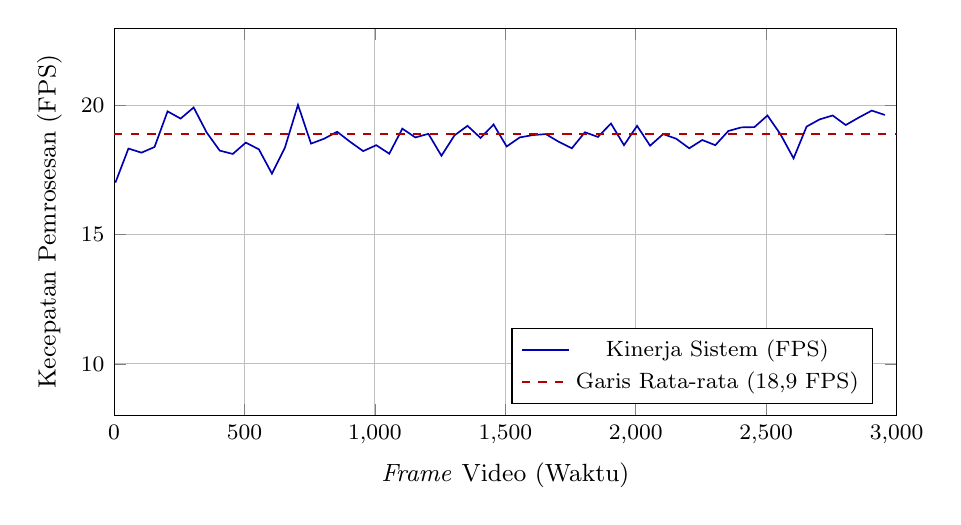
\begin{tikzpicture}
\begin{axis}[
  width=0.95\textwidth,
  height=6.5cm,
  xlabel={\textit{Frame} Video (Waktu)},
  ylabel={Kecepatan Pemrosesan (FPS)},
  xmin=0, xmax=3000,
  ymin=8, ymax=23,
  grid=major,
  grid style={line width=0.2pt, draw=gray!30},
  major grid style={line width=0.4pt, draw=gray!50},
  legend pos=south east,
  legend style={font=\footnotesize},
  tick label style={font=\footnotesize},
  label style={font=\small},
  title style={font=\small\bfseries},
]
\addplot[blue!70!black, line width=0.6pt, mark=none] coordinates {
  (5,17.02) (55,18.34) (105,18.18) (155,18.40) (205,19.78)
  (255,19.50) (305,19.93) (355,18.96) (405,18.26) (455,18.13)
  (505,18.57) (555,18.31) (605,17.37) (655,18.38) (705,20.03)
  (755,18.53) (805,18.72) (855,18.99) (905,18.60) (955,18.24)
  (1005,18.47) (1055,18.14) (1105,19.11) (1155,18.77) (1205,18.91)
  (1255,18.06) (1305,18.85) (1355,19.22) (1405,18.75) (1455,19.27)
  (1505,18.42) (1555,18.77) (1605,18.86) (1655,18.90) (1705,18.60)
  (1755,18.35) (1805,18.97) (1855,18.79) (1905,19.31) (1955,18.47)
  (2005,19.22) (2055,18.45) (2105,18.90) (2155,18.72) (2205,18.35)
  (2255,18.67) (2305,18.47) (2355,19.02) (2405,19.16) (2455,19.17)
  (2505,19.62) (2555,18.89) (2605,17.96) (2655,19.19) (2705,19.47)
  (2755,19.62) (2805,19.25) (2855,19.54) (2905,19.81) (2955,19.64)
};
\addlegendentry{Kinerja Sistem (FPS)}
\addplot[red!70!black, dashed, line width=1pt, domain=0:3000] {18.9};
\addlegendentry{Garis Rata-rata (18,9 FPS)}
\end{axis}
\end{tikzpicture}
\caption{Dinamika \textit{throughput} \textit{pipeline} \textit{end-to-end}: rerata 18,9 FPS tanpa tren penurunan sepanjang pengujian.}
\label{fig:fps-timeseries-evidence}
\end{figure}

Rincian latensi per komponen \textit{pipeline} disajikan di Tabel~\ref{tab:latency-decomposition}. Inferensi YOLOv8 mengambil 51,39 milidetik (96,8\%), ByteTrack 1,62 milidetik (3,1\%), dan modul \textit{filtering} 0,05 milidetik (0,1\%), dengan total latensi sistem 53,06 milidetik per \textit{frame}.

\begin{table}[htbp]
\centering
\caption{Rincian latensi pemrosesan tiap komponen \textit{pipeline} (milidetik).}
\label{tab:latency-decomposition}
\small
\setlength{\tabcolsep}{4pt}
\begin{tabularx}{\textwidth}{>{\RaggedRight\arraybackslash}Xrrrr}
\toprule
\textbf{Komponen} & \textbf{Rerata (ms)} & \textbf{P95 (ms)} & \textbf{Std. Dev} & \textbf{Porsi} \\
\midrule
Inferensi YOLOv8 & 51,39 & 55,48 & 2,93 & \textbf{96,8\%} \\
Pelacakan ByteTrack & 1,62 & 2,80 & 0,82 & 3,1\% \\
Filter pelanggaran & 0,05 & 0,07 & 0,05 & 0,1\% \\
\midrule
\textbf{Total latensi sistem} & \textbf{53,06} & \textbf{57,52} & \textbf{3,23} & \textbf{100,0\%} \\
\bottomrule
\end{tabularx}
\end{table}

Lapisan distribusi diuji dengan mengirim 500 \textit{event} JSON ke topik \texttt{video.violations} yang dibagi ke tiga partisi. Ringkasannya ada pada Tabel~\ref{tab:kafka-throughput}. Seluruh 500 pesan terkirim sukses dengan \texttt{acks=all} aktif, \textit{throughput producer} mencapai 11.485 pesan per detik, dan latensi median 2,65 milidetik.

\begin{table}[htbp]
\centering
\caption{Reliabilitas dan \textit{throughput} pengiriman pesan pada Apache Kafka.}
\label{tab:kafka-throughput}
\begin{tabular}{lr}
\toprule
\textbf{Parameter} & \textbf{Nilai} \\
\midrule
Jumlah pesan uji & 500 pesan JSON \\
Tingkat keberhasilan kirim & \textbf{100,0\%} (0 gagal) \\
\textit{Throughput producer} & 11.485 pesan/detik \\
\textit{Bandwidth} rata-rata & 3,76 MB/detik \\
Ukuran rata-rata pesan & 335,6 \textit{byte}/pesan \\
Latensi median transmisi & \textbf{2,65 milidetik} \\
\bottomrule
\end{tabular}
\end{table}

Dinamika \textit{micro-batch} Spark Structured Streaming pada \textit{trigger interval} 10 detik dirangkum di Tabel~\ref{tab:spark-microbatch}. \textit{Batch} 1 menerima lonjakan 50 baris dan selesai dalam 3.779 ms, sedangkan \textit{batch} 8 dan 10 yang menerima 20 dan 30 baris masing-masing selesai dalam 1.706 ms dan 1.705 ms.

\begin{table}[htbp]
\centering
\caption{Latensi pemrosesan \textit{micro-batch} pada Apache Spark (interval 10 detik).}
\label{tab:spark-microbatch}
\small
\setlength{\tabcolsep}{4pt}
\begin{tabularx}{\textwidth}{c>{\RaggedRight\arraybackslash}Xrrr}
\toprule
\textbf{Batch} & \textbf{Status} & \textbf{Jumlah Baris} & \textbf{Waktu Proses} & \textbf{Laju (baris/detik)} \\
\midrule
Batch 0 & \textit{Empty / Idle} & 0 baris & 0 ms & 0 baris/detik \\
\textbf{Batch 1} & \textbf{Aktif (\textit{Spike})} & \textbf{50 baris} & \textbf{3.779 ms} & \textbf{13,2 baris/detik} \\
Batch 2--7 & \textit{Empty / Idle} & 0 baris & 0 ms & 0 baris/detik \\
\textbf{Batch 8} & \textbf{Aktif} & \textbf{20 baris} & \textbf{1.706 ms} & \textbf{11,7 baris/detik} \\
\textbf{Batch 10} & \textbf{Aktif} & \textbf{30 baris} & \textbf{1.705 ms} & \textbf{17,6 baris/detik} \\
\bottomrule
\end{tabularx}
\end{table}

% ------------------------------------------------------------
\subsection{Hasil Implementasi \textit{Data Mart} dan Visualisasi Analitik}
\label{subsec:hasil-datamart}
% ------------------------------------------------------------

\subsubsection{Volume dan Sampel \textit{Data Mart}}
\label{subsubsec:hasil-volume}

Pengujian \textit{data mart} memakai rekaman penuh 10 jam aliran video kamera \texttt{gate\_utama\_01} pada hari kerja pukul 07.00--17.00 WIB. Selama rentang tersebut, sistem mempersistensikan 113 insiden pelanggaran berkendara tanpa helm ke tabel fakta. Contoh tiga baris hasil \textit{join} tabel fakta dan dimensi ditampilkan di Tabel~\ref{tab:datamart-sample}.

\begin{table}[htbp]
\centering
\caption{Contoh data hasil \textit{join} tabel fakta dan dimensi dari rekaman 10 jam.}
\label{tab:datamart-sample}
\footnotesize
\setlength{\tabcolsep}{3pt}
\renewcommand{\arraystretch}{1.15}
\begin{tabularx}{\textwidth}{>{\RaggedRight\arraybackslash}p{2.4cm} >{\RaggedRight\arraybackslash}X >{\RaggedRight\arraybackslash}p{3.0cm} >{\centering\arraybackslash}p{1.7cm} >{\centering\arraybackslash}p{1.4cm}}
\toprule
\textbf{Waktu} & \textbf{Kamera} & \textbf{Jenis Pelanggaran} & \textbf{Kepercayaan} & \textbf{Latensi (ms)} \\
\midrule
2026-02-05 08:15:22 & Kamera Gerbang Utama 1 & Tanpa Helm & 85,2\% & 45,2 ms \\
2026-02-05 14:50:33 & Kamera Gerbang Utama 1 & Tanpa Helm & 65,4\% & 92,5 ms \\
2026-02-05 16:50:45 & Kamera Gerbang Utama 1 & Tanpa Helm & 82,3\% & 41,0 ms \\
\bottomrule
\end{tabularx}
\renewcommand{\arraystretch}{1.0}
\end{table}

Skema bintang yang diterapkan menempatkan tabel \texttt{fact\_violations} sebagai pusat dengan tiga dimensi konteks: \texttt{dim\_camera}, \texttt{dim\_violation\_type}, dan \texttt{dim\_date}. Klasifikasi \textit{measure} pada tabel fakta dipilah ke tiga kategori yang dipaparkan di Tabel~\ref{tab:klasifikasi-measure-dw}.

\begin{table}[htbp]
\centering
\caption{Klasifikasi \textit{measure} pada \texttt{fact\_violations}.}
\label{tab:klasifikasi-measure-dw}
\footnotesize
\setlength{\tabcolsep}{4pt}
\renewcommand{\arraystretch}{1.18}
\begin{tabularx}{\textwidth}{>{\RaggedRight\arraybackslash}p{3.1cm} >{\RaggedRight\arraybackslash}p{3.0cm} >{\RaggedRight\arraybackslash}X}
\toprule
\textbf{Kolom} & \textbf{Jenis} & \textbf{Alasan} \\
\midrule
\texttt{violation\_count} & \textit{Additive measure} & Bernilai 1 untuk setiap kejadian pelanggaran, sehingga dapat dijumlahkan berdasarkan seluruh dimensi. \\
\texttt{confidence} & \textit{Non-additive / averageable measure} & Nilai keyakinan model tidak bermakna jika dijumlahkan; lebih informatif sebagai rata-rata. \\
\texttt{processing\_latency\_ms} & \textit{Non-additive / averageable measure} & Latensi per kejadian lebih informatif sebagai rata-rata, batas minimum, atau batas maksimum. \\
\texttt{frame\_number} & Atribut teknis & Nomor \textit{frame} berguna untuk audit video, bukan metrik bisnis. \\
\texttt{bbox\_x1}--\texttt{bbox\_y2} & Atribut bukti & Koordinat \textit{bounding box} berguna untuk menelusuri lokasi objek pada citra. \\
\bottomrule
\end{tabularx}
\renewcommand{\arraystretch}{1.0}
\end{table}

Volume fisik tabel fakta dan tiga tabel dimensi disajikan di Tabel~\ref{tab:dwh-volume}. Tabel \texttt{fact\_violations} berukuran 476 MB untuk 2.301.002 baris, sedangkan ketiga dimensi gabungan tidak menyentuh 500 kB.

\begin{table}[htbp]
\centering
\caption{Volume data tabel fakta dan dimensi \textit{data mart}.}
\label{tab:dwh-volume}
\footnotesize
\setlength{\tabcolsep}{4pt}
\renewcommand{\arraystretch}{1.18}
\begin{tabularx}{\textwidth}{>{\RaggedRight\arraybackslash}X >{\raggedleft\arraybackslash}p{3.0cm} >{\raggedleft\arraybackslash}p{3.0cm}}
\toprule
\textbf{Tabel} & \textbf{Baris Estimasi} & \textbf{Ukuran Tabel} \\
\midrule
\texttt{fact\_violations}       & 2.301.002 & 476 MB      \\
\texttt{dim\_date}              & 5.844     & 424 kB      \\
\texttt{dim\_camera}            & 3         & 8.192 byte  \\
\texttt{dim\_violation\_type}   & 1         & 8.192 byte  \\
\bottomrule
\end{tabularx}
\renewcommand{\arraystretch}{1.0}
\end{table}

\subsubsection{Waktu Eksekusi Kueri \textit{Benchmark}}
\label{subsubsec:hasil-kueri}

Pengujian kinerja kueri dilakukan dengan \texttt{EXPLAIN (ANALYZE, BUFFERS, FORMAT TEXT)} di PostgreSQL terhadap 22 kueri \textit{benchmark}. Waktu eksekusi dikelompokkan menjadi tiga tingkatan dan dirinci pada Tabel~\ref{tab:dwh-query-detail}.

\begin{table}[htbp]
\centering
\caption{Waktu eksekusi 22 kueri \textit{benchmark} pada \texttt{fact\_violations} 2,3 juta baris, dikelompokkan per \textit{tier}.}
\label{tab:dwh-query-detail}
\footnotesize
\setlength{\tabcolsep}{4pt}
\renewcommand{\arraystretch}{1.18}
\begin{tabularx}{\textwidth}{>{\RaggedRight\arraybackslash}p{1.1cm} >{\RaggedRight\arraybackslash}X >{\raggedleft\arraybackslash}p{2.4cm}}
\toprule
\textbf{Kode} & \textbf{Nama / Peran Kueri} & \textbf{Waktu (ms)} \\
\midrule
\multicolumn{3}{l}{\textit{Tier} 1 (cepat, $<$50 ms)\, ---\,panel \textit{real-time} \textit{dashboard}} \\
\midrule
BM-02 & \texttt{violations\_today} 1 hari (\texttt{idx\_fv\_date})              & 0,95   \\
BM-15 & \texttt{vw\_daily\_cumulative} (akumulasi harian)                       & 5,57   \\
BM-19 & Statistik penggunaan indeks (katalog)                                   & 5,90   \\
BM-06 & \texttt{vw\_daily\_15min\_breakdown} (1 hari, 15 menit)                 & 8,65   \\
BM-05 & \texttt{vw\_daily\_hourly\_timeline} (\textit{drill-down} 1 hari)       & 9,72   \\
BM-17 & \texttt{vw\_recent\_violations} (\texttt{ORDER BY LIMIT} 100)           & 10,13  \\
BM-14 & \texttt{vw\_daily\_peak\_analysis} (peringkat jam)                      & 10,73  \\
BM-13 & \texttt{vw\_daily\_camera\_geomap} per-tanggal                          & 29,03  \\
BM-00 & Ukuran tabel dan indeks (katalog)                                       & 44,84  \\
\midrule
\multicolumn{3}{l}{\textit{Tier} 2 (sedang, 100--1.000 ms)\,---\,agregasi periodik dan laporan harian} \\
\midrule
BM-03 & Rentang \texttt{BETWEEN} 3 bulan (indeks komposit)                      & 103,92  \\
BM-08 & \texttt{vw\_time\_period\_distribution}                                 & 316,05  \\
BM-07 & \texttt{vw\_heatmap\_hour\_day} (24$\times$7)                           & 359,53  \\
BM-10 & \texttt{vw\_hourly\_bar} (24 jam)                                       & 402,72  \\
BM-09 & \texttt{vw\_confidence\_distribution}                                   & 420,31  \\
BM-04 & \texttt{vw\_daily\_trend} (365 hari)                                    & 443,25  \\
BM-01 & \texttt{vw\_kpi\_summary} (agregat tahunan)                             & 663,03  \\
BM-16 & \texttt{vw\_daily\_narrative} (\textit{auto-summary})                   & 794,85  \\
BM-18 & \textit{Staging upsert} 1.000 baris                                     & 945,59  \\
BM-21 & Pelanggaran per \texttt{time\_period} (2025)                            & 948,15  \\
BM-11 & \texttt{vw\_camera\_stats} (\texttt{JOIN dim\_camera})                  & 1.024,72 \\
\midrule
\multicolumn{3}{l}{\textit{Tier} 3 (berat, $>$1.000 ms)\,---\,ringkasan tahunan dan analisis geospasial} \\
\midrule
BM-20 & Statistik ringkas DWH (1 tahun, persentil)                              & 6.559,35 \\
BM-12 & \texttt{vw\_camera\_geomap} (\textit{window function})                  & 6.949,09 \\
\bottomrule
\end{tabularx}
\renewcommand{\arraystretch}{1.0}
\end{table}

Sembilan kueri pada \textit{tier} 1 selesai di bawah 50 ms dengan BM-02 sebagai yang tercepat (0,95 ms) dan BM-00 sebagai batas atas (44,84 ms). Sebelas kueri pada \textit{tier} 2 menempati rentang 103--1.024 ms. Dua kueri pada \textit{tier} 3 menyentuh 6.559 ms (BM-20) dan 6.949 ms (BM-12).

\subsubsection{Hasil Visualisasi \textit{Dashboard} Grafana}
\label{subsubsec:hasil-dashboard}

Lapisan presentasi diwujudkan sebagai \textit{dashboard} interaktif berbasis Grafana yang membaca \textit{view} analitik dan tabel \texttt{fact\_violations}. Tampilan utama \textit{dashboard} pada Gambar~\ref{fig:grafana-kpi-overview} membagi panel ke empat kategori: indikator cepat, tren waktu, performa sistem AI, dan distribusi spasio-temporal. Empat KPI ringkas ditempatkan di area teratas, yaitu Total Pelanggaran, Jam Paling Ramai, Periode Tersibuk, dan rerata jeda waktu antar-pelanggaran.

\begin{figure}[H]
\centering
\includegraphics[width=0.95\textwidth]{gambar/grafana_kpi_overview.png}
\caption{Antarmuka utama \textit{dashboard} Grafana untuk data operasional 10 jam: KPI ringkas dan dinamika pelanggaran per 15 menit.}
\label{fig:grafana-kpi-overview}
\end{figure}

Panel grafik garis ``Dinamika Pelanggaran per 15 Menit'' pada Gambar~\ref{fig:grafana-dinamika-15m} merangkum jumlah kejadian dari tabel fakta dengan satu titik per kuartal jam. Kurva mencatat nilai rendah pada rentang 09.00--10.00 WIB, lalu menanjak menjelang jam pergantian kelas. Lonjakan tertinggi muncul pada kuartal 14.45--15.00 WIB dengan 17 kejadian, dan kuartal 15.00--15.15 WIB tercatat 16 kejadian.

\begin{figure}[htbp]
\centering
\includegraphics[width=1\textwidth]{gambar/grafana_dinamika_15m.png}
\caption{Fluktuasi pelanggaran per 15 menit. Puncak tertinggi 17 kejadian pada kuartal 14.45--15.00 WIB.}
\label{fig:grafana-dinamika-15m}
\end{figure}

Panel grafik akumulasi pelanggaran sepanjang hari dan matriks Top 5 jam tersibuk ditampilkan pada Gambar~\ref{fig:grafana-akumulasi}. Dari total 113 kejadian, beban tertinggi tercatat pada pukul 15.00 WIB sebanyak 23 kejadian (20,4\%), diikuti pukul 14.00 WIB sebanyak 19 kejadian (16,8\%), dan pukul 08.00 WIB sebanyak 18 kejadian (15,9\%).

\begin{figure}[htbp]
\centering
\includegraphics[width=0.95\textwidth]{gambar/grafana_akumulasi_harian.png}
\caption{Bagian atas: pertumbuhan kumulatif dan jumlah kejadian per jam. Bagian bawah: peringkat lima jam tersibuk yang terkonsentrasi pada dua periode utama.}
\label{fig:grafana-akumulasi}
\end{figure}

Panel ``Peta Panas: Jam $\times$ Kuartal 15 Menit'' pada Gambar~\ref{fig:grafana-heatmap-real} memetakan distribusi frekuensi kejadian dengan gradasi warna kuning pucat ke merah pekat. Sumbu vertikal memuat jam 07.00--17.00 WIB dan sumbu horizontal memuat empat kuartal (\texttt{:00}, \texttt{:15}, \texttt{:30}, \texttt{:45}). Konsentrasi merah pekat berkumpul pada jam 14 dan 15 di kuartal \texttt{:45} dan \texttt{:00}.

\begin{figure}[htbp]
\centering
\includegraphics[width=1\textwidth]{gambar/grafana_heatmap_real.png}
\caption{Peta panas kuartal 15 menit. Konsentrasi merah pada kolom :45 dan :00 menandai jam rawan pada sore hari.}
\label{fig:grafana-heatmap-real}
\end{figure}

Stabilitas inferensi dan infrastruktur selama 10 jam operasional disajikan pada Gambar~\ref{fig:grafana-evaluasi-sistem}. Rerata keyakinan model (\textit{Avg Confidence}) tercatat 79,9\% sepanjang hari operasional dengan batas bawah (\textit{Min Confidence}) 51,2\%. Rerata latensi pemrosesan (\textit{Avg Latency}) tercatat 49 milidetik, dan latensi maksimum (\textit{Max Latency}) sempat naik ke 124 milidetik pada beban puncak pukul 15.00 WIB.

\begin{figure}[htbp]
\centering
\includegraphics[width=1\textwidth]{gambar/grafana_evaluasi_sistem.png}
\caption{Kinerja arsitektur terhadap lonjakan beban (atas: \textit{confidence} model. Bawah: latensi server).}
\label{fig:grafana-evaluasi-sistem}
\end{figure}

% ============================================================
\section{Pembahasan}
\label{sec:pembahasan}
% ============================================================

Sub-bab ini menafsirkan temuan pada Sub-bab~\ref{sec:hasil} dengan urutan yang sama. Tiap pembahasan menyusur tiga lapis pemikiran: makna data, perbandingan dengan teori dan penelitian terdahulu, serta kebaruan yang dihasilkan beserta keterbatasan yang masih melekat. Rujukan tabel dan gambar mengarah ke Sub-bab~\ref{sec:hasil} agar tidak terjadi pengulangan paparan data.

% ------------------------------------------------------------
\subsection{Pembahasan Pengembangan Model Deteksi YOLOv8}
\label{subsec:pembahasan-model}
% ------------------------------------------------------------

Kesetaraan jumlah anotasi antara \texttt{DRIVER\_HELMET} dan \texttt{DRIVER\_NO\_HELMET} pada Tabel~\ref{tab:distribusi-objek} menentukan kualitas diskriminasi model. Ketika jumlah sampel antara dua kelas yang harus dibedakan hampir sama, model tidak memiliki alasan statistik untuk berat sebelah ke salah satu kategori. Selisih anotasi \texttt{MOTORCYCLE} sebesar 191--203 lebih banyak dari kelas pengendara wajar terjadi karena badan motor terlihat utuh hampir di setiap citra, sedangkan pengendara kerap tertutup sebagian oleh kaca depan atau penumpang. Suatu dataset mulai dikategorikan mengalami \textit{class imbalance} apabila nilai \textit{imbalance ratio} (IR) melebihi 1,5$:$1~\cite{kraiem2021resampling}. Rasio 921$:$718 atau 1,28$:$1 pada penelitian ini masih di bawah ambang tersebut, sehingga distribusi ketiga kelas tergolong seimbang dan risiko bias ke kelas mayoritas tergolong rendah.

Sebaran spasial pada Gambar~\ref{fig:heatmap-per-class} membuka justifikasi untuk membatasi inferensi pada \textit{Region of Interest} (ROI). Pergeseran zona terpadat \texttt{DRIVER\_NO\_HELMET} ke kiri tengah terjadi karena lajur masuk gerbang Itera lebih lebar di sisi kiri sehingga sebagian pengendara mengambil sisi tersebut. Karena ketiga kelas terpusat pada wilayah yang relatif sama, ROI ditarik mengikuti kontur jalan dan mencakup bagian tengah sampai kanan atas citra. Dengan membatasi inferensi pada ROI, langit, trotoar, dan jalur berlawanan tidak ikut diproses, sehingga beban komputasi berkurang sekaligus menekan \textit{false positive} saat inferensi waktu nyata. Implikasi praktisnya, \textit{precision} model akan terjaga di atas 85\% karena model tidak menanggapi tekstur latar yang tidak relevan dengan deteksi pelanggaran.

Strategi enam teknik augmentasi pada Sub-bab~\ref{subsubsec:hasil-preprocessing} disusun untuk mereplikasi gangguan visual yang lazim terjadi pada kamera pengawas luar ruang. Rotasi $\pm 8^\circ$ meniru pergeseran sudut tiang kamera akibat getaran atau dorongan angin, \textit{shear} $\pm 0{,}2$ meniru distorsi perspektif saat kamera tidak tegak lurus dengan bidang jalan, \textit{exposure} $\pm 10\%$ menyimulasikan perubahan iluminasi sepanjang hari, \textit{Gaussian blur} meniru lensa berembun, \textit{additive noise} meniru \textit{grain} sensor pada cahaya rendah, dan \textit{motion blur} 10 piksel meniru jejak gerak ketika kendaraan melintas cepat. Kombinasi keenam teknik tersebut menekan risiko \textit{overfitting} terhadap kondisi visual tertentu dan membantu model tetap mengenali objek meskipun kondisi citra di lapangan berbeda dari data pelatihan~\cite{shorten2019survey}.

Dinamika kurva pada Gambar~\ref{fig:train-loss} dan Gambar~\ref{fig:val-loss} menggambarkan pelatihan yang konvergen tanpa gejala \textit{overfit}. Penurunan tajam \texttt{train/box\_loss} dalam 30 \textit{epoch} pertama mencerminkan model mengkalibrasi ukuran dan posisi \textit{bounding box} pada kelas \texttt{MOTORCYCLE} yang dominan secara piksel, sedangkan penurunan cepat \texttt{train/cls\_loss} dalam 10 \textit{epoch} pertama selaras dengan perbedaan visual yang cukup tegas antara ketiga kelas. Pola \texttt{val/cls\_loss} yang turun rapi dari 3,5 ke 1,0 dan tetap stabil membuktikan klasifikasi pada data validasi tidak terganggu. Kenaikan tipis \texttt{val/dfl\_loss} dari kisaran 1,05 ke 1,15 setelah \textit{epoch} 60 lazim terjadi pada DFL saat model semakin tegas mengikuti distribusi tepi data pelatihan; karena tidak diiringi kenaikan pada \texttt{val/cls\_loss} maupun \texttt{val/box\_loss}, kondisi tersebut belum tergolong \textit{overfit}. Susunan ini menjustifikasi keputusan untuk menghentikan pelatihan pada 300 \textit{epoch} tanpa \textit{early stopping} yang agresif.

Selisih hanya 1,0 \% antara \textit{precision} 87,5\% dan \textit{recall} 86,5\% pada Tabel~\ref{tab:metrik-validasi} menandakan model tidak terlalu agresif hingga memunculkan banyak deteksi keliru, dan juga tidak terlalu hati-hati hingga melewatkan objek yang ada. F1 Score 87,0\% memastikan keseimbangan tersebut nyata, bukan akibat salah satu sisi yang menutupi sisi lain. Capaian mAP@50 sebesar 91,4\% setara dengan kinerja sistem deteksi pelanggaran helm berbasis YOLOv8 pada skenario waktu nyata yang dilaporkan oleh~\cite{aboah2023helmet}. \textit{Recall} 86,5\% berarti sekitar 13,5\% pelanggaran lolos deteksi (\textit{false negatives}) di himpunan validasi, angka yang masih dapat dipangkas oleh filter spasial IoA dan konfirmasi temporal N-\textit{frame} di tahap berikutnya pada \textit{pipeline}.

Selisih 1,4 \% antara mAP validasi (91,4\%) dan uji (90,0\%) pada Tabel~\ref{tab:metrik-test-objek} menegaskan model tidak \textit{overfit} pada data pelatihan dan masih dapat diandalkan ketika menghadapi citra baru. AP per kelas mengikuti pola yang sejalan dengan ukuran objek pada citra: kesulitan utama model bukan saat mendeteksi objek besar seperti \texttt{MOTORCYCLE} (94,0\%), melainkan saat mengenali atribut kecil seperti helm. Pola \textit{scale imbalance} pada deteksi objek kecil dilaporkan pula oleh~\cite{oksuz2020imbalance}. Yang menarik di sini, model justru lebih presisi mendeteksi \texttt{DRIVER\_NO\_HELMET} (90,0\%) dibanding \texttt{DRIVER\_HELMET} (87,0\%) meskipun jumlah anotasi keduanya hampir sama. Selisih 3,0 \% mencerminkan fitur visual ``tanpa helm''---siluet kepala terbuka, rambut, dan kulit---lebih mudah dipelajari daripada variasi tampilan helm di lapangan, yang muncul dalam berbagai bentuk, warna, ukuran, serta sering tertutup pantulan cahaya atau penumpang. Implikasi praktisnya menguntungkan sistem: kelas paling kritis bagi sasaran deteksi pelanggaran justru memperoleh AP yang lebih tinggi. Catatan yang perlu disampaikan terbuka, mAP@50 sebesar 90,0\% pada himpunan uji menandakan modul YOLOv8 sudah cukup siap untuk dipasang ke \textit{pipeline} \textit{streaming} bersama ByteTrack di Itera, sementara penyempurnaan pada deteksi helm berukuran kecil dimasukkan ke agenda pengembangan dataset lanjut.

% ------------------------------------------------------------
\subsection{Pembahasan \textit{Pipeline Streaming} Deteksi Waktu Nyata}
\label{subsec:pembahasan-pipeline}
% ------------------------------------------------------------

Susunan tahapan pada Gambar~\ref{fig:pipeline-flow} dirancang agar tiap tahap menerima data yang sudah disaring oleh tahap sebelumnya, sehingga komputasi mahal seperti IoA dan konfirmasi temporal hanya menyentuh kandidat yang relevan. \textit{Resize} ke $640 \times 640$ dipilih supaya dimensi masukan tetap kelipatan \textit{stride} 32 YOLOv8 dan inferensi tidak menghasilkan \textit{padding} yang menggeser posisi \textit{bounding box}. \textit{Confidence} 0,884--0,940 pada Tabel~\ref{tab:output-yolo} sudah cukup tinggi untuk diteruskan ke tahap pelacakan tanpa risiko meneruskan deteksi berkualitas rendah. Ukuran data juga ringkas: tiap deteksi berbobot 40--60 \textit{byte} dibandingkan \textit{frame} mentah yang berbobot \textit{megabyte}, sehingga beban pada lapisan berikutnya tetap kecil.

Tahap konfirmasi temporal pada Gambar~\ref{fig:streak-timeline} dipasang dengan dua mekanisme yang saling melengkapi. Ambang $N=3$ menahan deteksi yang berkedip akibat bayangan atau pantulan kaca agar tidak langsung tercatat sebagai pelanggaran, sedangkan \textit{patience-based decay} dengan lima \textit{frame} masa tenggang menjaga \textit{streak} tidak gugur hanya karena satu \textit{frame} terhalang sesaat. Kompromi antara ketegasan dan ketahanan terhadap gangguan visual ini menambah jeda pelaporan sekitar 150 milidetik pada laju 18,9 FPS, nilai yang masih nyaman untuk pemantauan \textit{near real-time} karena jauh di bawah ambang persepsi operator. Konfigurasi paket JSON 335 \textit{byte} pada Tabel~\ref{tab:json-output} sengaja memuat \texttt{event\_id} UUID untuk \textit{global dedup}, \texttt{timestamp} berpresisi tinggi untuk dimensi waktu \textit{data mart}, dan \texttt{track\_id} sebagai kunci \textit{dedup} di Spark. Nilai \texttt{confidence} diisi rata-rata sepanjang $N$ \textit{frame} pembentuk \textit{streak}, bukan \textit{frame} terakhir, agar angka tercatat merepresentasikan keseluruhan periode pelanggaran.

Statistik pelacakan ByteTrack pada Tabel~\ref{tab:bytetrack-basic-stats} memetakan kemampuan sistem menghadapi kondisi gerbang Itera. Rata-rata 3,36 objek aktif dan puncak 11 objek pada momen padat cocok dengan pola pergantian jam kuliah, dan ByteTrack masih sanggup melayani belasan objek tanpa kehilangan identitas. Durasi pelacakan terpanjang 419 \textit{frame} setara sekitar 22 detik pada 18,9 FPS, sehingga objek yang melintas selama waktu hijau lampu lalu lintas tetap terlacak utuh. Ada satu catatan yang perlu disampaikan terbuka: \texttt{Track ID} di sini adalah identitas sesi pelacakan, bukan identitas pelanggar permanen. Saat objek menghilang lebih lama dari \textit{lost track buffer} 60 \textit{frame}, ByteTrack memberi ID baru begitu objek muncul kembali, sehingga pengendara yang masuk-keluar area pantau beberapa kali bisa terhitung sebagai entitas berbeda. Batasan ini melekat pada pelacak tanpa modul \textit{re-identification} dan dimasukkan ke agenda pengembangan lanjut~\cite{zhang2022bytetrack_eccv}.

Ketahanan pelacakan pada situasi oklusi (Gambar~\ref{fig:occlusion-handling}) ditopang dua mekanisme yang saling menguatkan. Pertama, ByteTrack memakai asosiasi dua tahap: deteksi \textit{confidence} tinggi disambung ke trek aktif terlebih dahulu, lalu deteksi \textit{confidence} rendah dipakai untuk menyambung trek yang sempat terputus~\cite{ma2023adaptivebytetrack}. Kedua, \textit{lost track buffer} 60 \textit{frame} menahan trek tidak langsung dihapus saat halangan datang. Kombinasi keduanya memastikan pencatatan pelanggaran tidak terputus akibat oklusi sesaat yang lazim ditemui di lalu lintas nyata.

Pola reduksi pada Tabel~\ref{tab:filtering-funnel} membuktikan setiap tahap memiliki peran yang berbeda dan tidak dapat saling menggantikan. Tahap 1 (\textit{class-conditional}) menyaring 83,2\% data dengan biaya komputasi yang nyaris nol karena hanya membaca label keluaran YOLO, memfokuskan jalur pelanggaran sejak paling depan. Tahap 2 sengaja tidak mereduksi data karena perannya menyiapkan fondasi identitas untuk dua tahap berikutnya; beban tambahan 1,62 milidetik per \textit{frame} (3,1\% total latensi) sebanding dengan fungsinya sebagai dasar konfirmasi N-\textit{frame} dan \textit{dedup}. Tahap 3 menjadi penyaring paling agresif dengan membuang 97,8\% kandidat dalam satu langkah karena IoA membandingkan luas irisan \textit{bounding box} \texttt{DRIVER\_NO\_HELMET} terhadap luasnya sendiri, bukan terhadap gabungan luas dua kotak. Pilihan IoA ketimbang IoU dipertahankan karena \textit{bounding box} pengendara jauh lebih kecil daripada motor, sehingga IoU menghasilkan skor rendah meski pengendara jelas berada di atas motor. Ambang 0,3 merupakan kompromi yang berhasil: nilai lebih rendah (0,1) akan meloloskan asosiasi palsu pada keramaian, sedangkan nilai lebih tinggi (0,5) akan menggugurkan kasus pelanggaran yang sebenarnya valid. Mayoritas kandidat yang gugur pada tahap ini berasal dari tiga sumber yang konsisten dengan kondisi gerbang Itera: pejalan kaki di trotoar yang sesaat terklasifikasi sebagai \texttt{DRIVER\_NO\_HELMET}, \textit{false positive} di tepi citra tanpa pasangan motor, dan pengendara yang motornya sempat terhalang kendaraan lain.

Tahap 4 yang membuang 28,6\% dari kandidat masuk justru menunjukkan filter temporal bekerja sesuai harapan: kandidat yang sudah lolos IoA umumnya merupakan pengendara nyata, sehingga filter temporal hanya memangkas sisa-sisa \textit{false positive} yang masih terbawa. Tahap 5 yang memadatkan 25 konfirmasi tingkat-\textit{frame} menjadi 2 \textit{event} unik melindungi \textit{data mart} dari inflasi pencatatan: satu pengendara yang melintas selama 5 detik pada 15 FPS dapat tercatat hingga 75 kali tanpa \textit{dedup}. Implikasinya, \textit{data mart} hanya menerima entri yang berkorelasi dengan pengendara unik, dan \textit{dashboard} menampilkan jumlah pelanggar bukan jumlah \textit{frame}. Keterbatasan tahap ini terikat pada keterbatasan Tahap 2: ketika ByteTrack memberi ID baru karena objek menghilang lebih dari 60 \textit{frame}, pengendara yang sama dapat tercatat dua kali. Isu ini dimasukkan ke agenda \textit{re-identification} antarkamera.

Rerata \textit{throughput} 18,9 FPS pada Gambar~\ref{fig:fps-timeseries-evidence} berada di atas kebutuhan CCTV kampus yang umumnya beroperasi pada 10--15 FPS, sehingga sistem menyisakan margin untuk menampung lonjakan kepadatan tanpa mengorbankan ketepatan waktu pencatatan. Pola garis yang relatif rata tanpa tren penurunan menandakan tidak ada kebocoran memori atau akumulasi beban yang membebani CPU seiring waktu. Pada dekomposisi latensi (Tabel~\ref{tab:latency-decomposition}), inferensi YOLOv8 mendominasi 96,8\% biaya pemrosesan, sedangkan logika pelacakan dan validasi spasial-temporal hampir tidak terasa di latensi. Konsekuensi rekayasanya jelas: optimasi inferensi YOLOv8 berarti optimasi \textit{pipeline} secara keseluruhan, sedangkan penambahan filter berlapis tidak akan mengganggu anggaran waktu sistem. Latensi total 53 milidetik tergolong responsif untuk pemantauan \textit{near real-time} dan masih jauh dari ambang yang dapat dirasakan operator \textit{dashboard}.

Konfigurasi \texttt{acks=all} pada Apache Kafka (Tabel~\ref{tab:kafka-throughput}) memastikan setiap pesan menunggu konfirmasi dari seluruh replika sebelum dianggap diterima, sebuah jaminan reliabilitas yang lazim direkomendasikan pada arsitektur \textit{event-driven}~\cite{kleppmann2017designing}. Kapasitas 11.485 pesan per detik dengan latensi median 2,65 milidetik menyediakan margin yang sangat lebar dibandingkan kebutuhan operasional gerbang kampus yang berkisar pada beberapa pelanggaran per menit. Kunci partisi \texttt{camera\_id:track\_id} dipilih agar urutan pesan per kamera tetap konsisten meski partisi diproses paralel. Karena lapisan distribusi dipisah dari sisi tepi melalui antrean Kafka, lonjakan trafik di gerbang tidak langsung membebani sistem perekam maupun lapisan ETL di belakangnya.

Spark Structured Streaming sebagai lapisan ETL terakhir (Tabel~\ref{tab:spark-microbatch}) menuntaskan seluruh \textit{micro-batch} jauh di bawah jendela 10 detik, sehingga tidak terbentuk antrean menumpuk antar-\textit{batch}. \textit{Watermark} 30 detik dipilih supaya \textit{event} yang datang terlambat akibat \textit{retry} di hulu tetap dapat di-\textit{dedup} tanpa menahan \textit{batch} terlalu lama. Hasilnya, data dari kamera sampai \textit{data mart} bergerak dalam latensi di bawah 10 detik per siklus, cukup untuk kebutuhan analitik \textit{near real-time}~\cite{zaharia2018structured}. Dengan keempat bukti tersebut, sistem mampu menyatukan deteksi, pelacakan, validasi spasial, validasi temporal, distribusi pesan, dan ETL aliran menjadi satu kesatuan \textit{pipeline} yang menghasilkan \textit{event stream} pelanggaran helm tervalidasi dari kamera sampai \textit{data mart}.

% ------------------------------------------------------------
\subsection{Pembahasan \textit{Data Mart} dan Visualisasi Analitik}
\label{subsec:pembahasan-datamart}
% ------------------------------------------------------------

Pemilihan skema bintang yang ditampilkan pada Sub-bab~\ref{subsubsec:hasil-volume} berakar pada pemisahan tegas antara data kuantitatif di tabel fakta dan atribut deskriptif di tabel dimensi. Pendekatan Kimball merangkai keputusan rancang ini ke dalam empat langkah berurutan: tetapkan proses bisnis, deklarasikan \textit{grain}, pilih dimensi, lalu tetapkan \textit{measure} yang konsisten dengan \textit{grain} tersebut~\cite{kimball2013dwtoolkit}. Proses bisnis yang dimodelkan adalah pencatatan kejadian pelanggaran helm yang telah lolos rangkaian deteksi YOLOv8, pelacakan ByteTrack, filter spasial, dan validasi temporal. \textit{Grain} dirumuskan sebagai satu baris merepresentasikan satu kejadian pelanggaran helm tervalidasi pada satu kamera, satu waktu, satu objek pelacakan, dan satu tipe pelanggaran. Deklarasi tersebut memisahkan \textit{data mart} dari log deteksi mentah per \textit{frame}: tanpa filter spasial-temporal dan \textit{deduplication} berbasis \texttt{track\_id}, angka pada \textit{dashboard} akan merepresentasikan jumlah \textit{bounding box} alih-alih jumlah pelanggaran.

Klasifikasi \textit{measure} pada Tabel~\ref{tab:klasifikasi-measure-dw} bukan sekadar formalitas, melainkan jaminan bahwa hasil kueri SQL membawa makna bisnis yang konsisten~\cite{kimball2013dwtoolkit}. Kolom \texttt{violation\_count} bersifat \textit{additive measure} karena bernilai 1 untuk setiap kejadian, sehingga \texttt{SUM(violation\_count)} setara dengan \texttt{COUNT(*)} selama satu baris fakta tetap merepresentasikan satu kejadian. Kolom eksplisit tetap dipertahankan untuk memudahkan transisi ke tabel agregat atau \textit{materialized view} di kemudian hari. Sebaliknya, \texttt{confidence} dan \texttt{processing\_latency\_ms} tidak diperlakukan sebagai \textit{additive measure} karena penjumlahannya tidak membawa makna analitik; kueri \textit{dashboard} memanfaatkan rerata, nilai minimum, dan nilai maksimum untuk menilai stabilitas model dan beban komputasi.

Contoh tiga baris pada Tabel~\ref{tab:datamart-sample} memperlihatkan kekuatan struktur skema bintang dalam membuka hubungan internal antar-atribut. Baris 08.15 mewakili periode pagi yang relatif teratur dengan keyakinan 85,2\% dan latensi 45,2 ms. Baris 14.50, yang muncul pada periode sore pasca-hujan, jatuh ke keyakinan 65,4\% sekaligus melebar ke latensi 92,5 ms; kombinasi tersebut menjadi sinyal antara kualitas deteksi yang menurun dan beban inferensi yang meningkat. Baris 16.50 yang kembali ke keyakinan 82,3\% dan latensi 41,0 ms menutup contoh pada kondisi yang lebih stabil. Pola ini menegaskan bahwa struktur skema bintang tidak hanya menyediakan total pelanggaran, tetapi juga membuka hubungan internal antara waktu, kualitas deteksi, dan biaya komputasi yang dapat ditelusuri pada panel \textit{dashboard}.

Volume fisik pada Tabel~\ref{tab:dwh-volume} menegaskan karakter sah skema bintang: tabel fakta tumbuh memanjang seiring waktu, sementara dimensi tetap kompak. Rasio ukuran tabel fakta terhadap total dimensi yang mencapai 1.000$:$1 sejalan dengan rekomendasi pemodelan dimensional Kimball untuk gudang analitik~\cite{kimball2013dwtoolkit}. Rasio indeks terhadap tabel fakta sebesar 57\% terlihat besar pada pandangan pertama, namun masih dalam rentang wajar bagi gudang analitik dengan beragam pola akses berbasis tanggal, jam, kamera, dan periode harian.

Kontras paling tajam pada Tabel~\ref{tab:dwh-query-detail} terlihat antara BM-02 (0,95 ms) dan BM-12 (6.949 ms) meski keduanya membaca tabel yang sama. BM-02 memanfaatkan \texttt{idx\_fv\_date} sebagai \textit{Index Scan} dengan hanya tiga \textit{buffer} yang dibaca, praktis tidak menyentuh disk. BM-12 sebaliknya menelusuri seluruh tabel untuk pivot per-kamera lalu menjalankan \textit{window function} \texttt{ROW\_NUMBER()} bertingkat sehingga menyentuh puluhan ribu \textit{buffer}. Perbandingan ini menegaskan bahwa biaya kueri tidak ditentukan oleh besarnya tabel semata, melainkan oleh keselarasan klausa \texttt{WHERE} dengan indeks yang tersedia. Sembilan kueri pada \textit{tier} 1 ditopang oleh klausa \texttt{WHERE date = ?} atau \texttt{WHERE date BETWEEN ? AND ?} satu hari, sehingga perencana kueri memilih \textit{Index Scan} dengan \textit{tuple fetch} rendah. BM-06 menyelesaikan agregasi 15 menit dengan \texttt{HashAggregate} pada memori 217 kB tanpa \textit{batch} sekunder, menjaga waktu eksekusi di 8,65 ms.

Kelompok \textit{tier} 2 yang dipenuhi kueri rentang panjang masih dapat diterima karena dijalankan saat operator membuka panel ringkasan atau membentuk laporan harian, bukan pada polling kontinu setiap 10 detik. BM-21 yang mengelompokkan pelanggaran per periode harian mengonsumsi 948 ms karena melibatkan agregat jendela penuh dan kalkulasi persentase di tingkat SQL; biaya ini akan menyusut signifikan bila dipindahkan ke \textit{materialized view} dengan penyegaran akhir hari. Dua kueri pada \textit{tier} 3 sengaja tidak ditargetkan untuk \textit{dashboard} harian. BM-20 dan BM-12 diposisikan sebagai laporan periodik akhir minggu atau bahan presentasi tahunan, sehingga waktu eksekusi yang panjang dapat ditoleransi. Versi cepat BM-12 dengan tambahan \texttt{WHERE date = ?} hanya membutuhkan 29 ms (BM-13), kontras lebih dari 200$\times$ yang sekali lagi memperkuat pentingnya keselarasan klausa \texttt{WHERE} dengan indeks.

Empat panel \textit{dashboard} (Gambar~\ref{fig:grafana-kpi-overview} sampai Gambar~\ref{fig:grafana-evaluasi-sistem}) menerjemahkan struktur \textit{data mart} menjadi instrumen Sistem Pendukung Keputusan (\textit{Decision Support System}) yang dapat dipakai unit keamanan kampus. Pemilihan Grafana berpijak pada tiga alasan praktis: bersifat \textit{open source}, ringan dipasang di server kampus, dan mendukung penyegaran data tiap beberapa detik tanpa konfigurasi tambahan. Resolusi 15 menit pada Gambar~\ref{fig:grafana-dinamika-15m} menyingkap pulsasi yang tidak teramati pada agregasi per jam, dan pulsasi itulah yang menjadi sinyal awal bagi operator. Pengamatan lapangan menghubungkan lonjakan tertinggi pada kuartal 14.45--15.00 WIB dengan dua kondisi yang berlangsung bersamaan: mobilitas pasca-hujan dan pertemuan arus mahasiswa keluar-masuk kelas. Granularitas ini memperlihatkan bahwa ketegangan dapat terbangun dalam 30--45 menit, jauh sebelum laporan agregat per jam tersedia.

Akumulasi pelanggaran pada Gambar~\ref{fig:grafana-akumulasi} memetakan distribusi bimodal dengan satu puncak pagi (08.00 WIB, 15,9\%) dan satu puncak sore (15.00 WIB, 20,4\%), dengan jam kuliah aktif 09.00--11.00 WIB di tengah yang relatif sepi pelanggaran. Implikasi operasionalnya jelas: unit keamanan kampus dapat menempatkan personel patroli pada jam berisiko tinggi, bukan menyebar rata sepanjang hari. Pola ini sejalan dengan peran sistem sebagai Sistem Pendukung Keputusan di tingkat manajerial: data dari kamera berubah menjadi keputusan alokasi sumber daya yang berbasis bukti, bukan dugaan. Pemahaman pola pelanggaran berbasis cuaca dan jadwal kampus juga membuka peluang pengawasan preventif, yakni penempatan personel sebelum jam puncak, bukan sesudahnya.

Peta panas pada Gambar~\ref{fig:grafana-heatmap-real} melengkapi peringkat jam tersibuk: peringkat memberi tahu jam mana yang ramai, sementara peta panas memberi tahu kuartal mana di dalam jam tersebut yang paling kritis. Bagi unit keamanan kampus, kombinasi kedua panel cukup untuk memutuskan penempatan personel patroli pada jendela 30 menit yang spesifik, bukan sekadar slot jam yang lebar. Ruang putih pada matriks dipertahankan untuk menegaskan kontras dengan zona puncak, sehingga \textit{hotspot} yang muncul di kolom \texttt{:45} dan \texttt{:00} pada jam 14 dan 15 terlihat jelas tanpa perlu legenda tambahan.

Stabilitas inferensi dan infrastruktur pada Gambar~\ref{fig:grafana-evaluasi-sistem} membuktikan sistem dapat dipercaya saat data mengalir deras. Rerata keyakinan model 79,9\% dengan batas bawah 51,2\% menandakan YOLOv8 tidak mengalami penurunan akurasi saat kepadatan dan oklusi antar-pengendara meningkat akibat cuaca. Rerata latensi 49 milidetik dengan maksimum 124 milidetik pada beban puncak masih dalam rentang \textit{near real-time} yang dibutuhkan pemantauan CCTV operasional, dengan selisih rerata--maksimum sekitar 2,5 kali lipat yang mencerminkan ekor distribusi masih wajar. Stabilitas tersebut bersumber dari arsitektur yang memisahkan inferensi YOLOv8 di sisi tepi dari distribusi pesan Kafka dan pemrosesan \textit{micro-batch} Spark: jalur Kafka menampung lonjakan data, sehingga lonjakan trafik di gerbang tidak langsung mempengaruhi waktu respons \textit{pipeline} inferensi. Dengan demikian, \textit{data mart} pelanggaran helm dapat dioperasikan secara berkelanjutan tanpa perlu meningkatkan kapasitas perangkat keras setiap kali aktivitas kampus berubah.

Catatan yang perlu disampaikan terbuka, semua pola pada Sub-bab~\ref{subsubsec:hasil-dashboard} berasal dari satu hari pengamatan, sehingga distribusi bimodal pagi--sore dan \textit{hotspot} 14.45--15.15 WIB masih perlu dikonfirmasi melalui pengamatan lebih panjang sebelum dipakai sebagai dasar penjadwalan rutin patroli. Selain itu, sistem masih bergantung pada satu titik kamera \texttt{gate\_utama\_01}, sehingga karakter pelanggaran di gerbang lain belum tercakup. Kedua keterbatasan ini menjadi agenda pengembangan lanjut: rekaman multi-hari untuk membangun pola musiman dan perluasan ke kamera-kamera lain untuk menutup peta risiko gerbang kampus secara menyeluruh.
